\documentclass[a4paper]{article}
\usepackage[affil-it]{authblk}
\usepackage[backend=bibtex,style=numeric]{biblatex}
\usepackage{amsmath}
\usepackage{amssymb}
\usepackage{graphicx}
\usepackage{geometry}
\geometry{margin=1.5cm, vmargin={0pt,1cm}}
\setlength{\topmargin}{-1cm}
\setlength{\paperheight}{29.7cm}
\setlength{\textheight}{25.3cm}

\addbibresource{citation.bib}

\begin{document}
% =================================================
\title{Numerical Analysis homework \# 3}
\author{Wang Hengning 3230104148
  \thanks{Electronic address: \texttt{whning@zju.edu.cn}}}
\affil{Computational mathematics 2301, Zhejiang University }

% 使用PDF中的截止日期
\date{Due time: November 11, 2025}

\maketitle

% ============================================

\section*{Problem I: Determining $p(x)$ for a $C^2$ cubic spline $s(x)$}

Let $s_0(x) = p(x) = ax^3 + bx^2 + cx + d$ on $[0, 1]$ and $s_1(x) = (2-x)^3$ on $[1, 2]$.
The condition $s(0) = p(0) = 0$ implies $d=0$.
The spline $s \in \mathbb{S}_3^2$ requires $C^2$ continuity at $x=1$.

For $p(x) = ax^3 + bx^2 + cx$:
\[ p'(x) = 3ax^2 + 2bx + c, \quad p''(x) = 6ax + 2b \]
For $s_1(x) = (2-x)^3$:
\[ s_1'(x) = -3(2-x)^2, \quad s_1''(x) = 6(2-x) \]

At $x=1$, the values for $s_1$ are $s_1(1) = 1$, $s_1'(1) = -3$, and $s_1''(1) = 6$.
The $C^2$ continuity conditions $p^{(k)}(1) = s_1^{(k)}(1)$ for $k=0, 1, 2$ yield the system:
\[ \begin{cases} p(1) = a + b + c = 1 \\ p'(1) = 3a + 2b + c = -3 \\ p''(1) = 6a + 2b = 6 \end{cases} \]
Solving this system gives $a=7$, $b=-18$, and $c=12$.
\[ p(x) = 7x^3 - 18x^2 + 12x \]
---
A natural cubic spline requires $s''(x) = 0$ at the endpoints $x=0$ and $x=2$.
\[ s''(2) = s_1''(2) = 0 \]
\[ s''(0) = p''(0) = 6a(0) + 2b = 2(-18) = -36 \]
Since $s''(0) = -36 \neq 0$, $s(x)$ is \textbf{not} a natural cubic spline.


\section*{Problem II: Interpolating with a quadratic spline $s \in \mathbb{S}_2^1$}

(a)
A quadratic spline $s \in \mathbb{S}_2^1$ on $n$ knots $x_1, \dots, x_n$ consists of $n-1$ quadratic pieces $s_i \in \mathbb{P}_2$.
Each piece has 3 coefficients, giving $3(n-1)$ total degrees of freedom (DoF).
The constraints are:
\begin{enumerate}
  \item Interpolation: $s_i(x_i) = f_i$ and $s_i(x_{i+1}) = f_{i+1}$ for $i=1, \dots, n-1$. ($2(n-1)$ conditions)
  \item $C^1$ continuity: $s'_{i-1}(x_i) = s'_i(x_i)$ at the $n-2$ interior knots $x_2, \dots, x_{n-1}$. ($n-2$ conditions)
\end{enumerate}
Total constraints: $2(n-1) + (n-2) = 3n-4$.
Free parameters: $\text{DoF} - \text{Constraints} = (3n-3) - (3n-4) = 1$.
Therefore, one additional condition is needed to determine $s$ uniquely.

---
(b)
Represent $p_i(x) = s|_{[x_i, x_{i+1}]} \in \mathbb{P}_2$ centered at $x_i$:
\[ p_i(x) = c_0 + c_1(x-x_i) + c_2(x-x_i)^2 \]
\[ p_i'(x) = c_1 + 2c_2(x-x_i) \]
The conditions $p_i(x_i) = f_i$ and $p_i'(x_i) = m_i$ yield $c_0 = f_i$ and $c_1 = m_i$.
Let $h_i = x_{i+1} - x_i$. The condition $p_i(x_{i+1}) = f_{i+1}$ determines $c_2$:
\[ f_i + m_i h_i + c_2 h_i^2 = f_{i+1} \implies c_2 = \frac{f_{i+1} - f_i - m_i h_i}{h_i^2} \]
\[ p_i(x) = f_i + m_i(x-x_i) + \left( \frac{f_{i+1} - f_i - m_i h_i}{h_i^2} \right) (x-x_i)^2 \]

---
(c)
The $C^1$ continuity $s'_{i-1}(x_i) = s'_i(x_i) = m_i$ is required for $i=2, \dots, n$.
Let $h_{i-1} = x_i - x_{i-1}$. Using the result from (b) for $p_{i-1}(x)$:
\[ p'_{i-1}(x) = m_{i-1} + 2 \left( \frac{f_i - f_{i-1} - m_{i-1} h_{i-1}}{h_{i-1}^2} \right) (x - x_{i-1}) \]
Evaluating at $x = x_i$:
\begin{align*}
p'_{i-1}(x_i) &= m_{i-1} + 2 \left( \frac{f_i - f_{i-1} - m_{i-1} h_{i-1}}{h_{i-1}^2} \right) h_{i-1} \\
&= m_{i-1} + \frac{2(f_i - f_{i-1})}{h_{i-1}} - 2m_{i-1} = -m_{i-1} + \frac{2(f_i - f_{i-1})}{h_{i-1}}
\end{align*}
The continuity condition $m_i = p'_{i-1}(x_i)$ gives the recurrence relation for $i=2, \dots, n$:
\[ m_i = -m_{i-1} + \frac{2(f_i - f_{i-1})}{h_{i-1}} \]
Given $m_1 = f'(a)$, $m_2$ can be computed, then $m_3$, and so on, sequentially determining $m_2, \dots, m_n$.


\section*{Problem III: Determining a natural cubic spline $s(x)$}

Let $s_1(x) = 1 + c(x+1)^3$ on $[-1, 0]$ and $s_2(x) = ax^3 + bx^2 + dx + e$ on $[0, 1]$.
The spline must be $C^2$ continuous at $x=0$ and satisfy $s''(-1) = 0$ and $s''(1) = 0$.

Derivatives for $s_1(x)$:
\[ s'_1(x) = 3c(x+1)^2, \quad s''_1(x) = 6c(x+1) \]
The condition $s''(-1) = s''_1(-1) = 0$ is satisfied for any $c \in \mathbb{R}$.

Derivatives for $s_2(x)$:
\[ s'_2(x) = 3ax^2 + 2bx + d, \quad s''_2(x) = 6ax + 2b \]
Continuity at $x=0$, $s_1^{(k)}(0) = s_2^{(k)}(0)$, determines $e, d, b$ in terms of $c$:
\begin{align*}
C^0: \quad & s_1(0) = 1+c \implies s_2(0) = e = 1+c \\
C^1: \quad & s'_1(0) = 3c \implies s'_2(0) = d = 3c \\
C^2: \quad & s''_1(0) = 6c \implies s''_2(0) = 2b = 6c \implies b = 3c
\end{align*}
So, $s_2(x) = ax^3 + 3cx^2 + 3cx + (1+c)$.
The remaining natural condition $s''(1) = s''_2(1) = 0$ gives:
\[ s''_2(1) = 6a(1) + 2b = 6a + 2(3c) = 6a + 6c = 0 \implies a = -c \]
This determines $s_2(x)$:
\[ s_2(x) = -cx^3 + 3cx^2 + 3cx + (1+c) = c(-x^3 + 3x^2 + 3x + 1) + 1 \]
---
To find $c$, use the condition $s(1) = -1$:
\[ s(1) = s_2(1) = c(-1 + 3 + 3 + 1) + 1 = 6c + 1 \]
\[ 6c + 1 = -1 \implies 6c = -2 \implies c = -\frac{1}{3} \]


\section*{Problem IV: Natural cubic spline interpolation of $f(x) = \cos(\frac{\pi x}{2})$}

(a)
The function is $f(x) = \cos(\frac{\pi x}{2})$ on $[-1, 1]$.
The knots are $x_1 = -1$, $x_2 = 0$, $x_3 = 1$. The data is:
\[ f_1 = f(-1) = 0, \quad f_2 = f(0) = 1, \quad f_3 = f(1) = 0 \]
Let $s(x)$ be the spline ($s_1$ on $[-1, 0]$, $s_2$ on $[0, 1]$) and $M_i = s''(x_i)$.
Natural boundary conditions: $M_1 = 0$, $M_3 = 0$.
Knot spacing: $h_1 = x_2 - x_1 = 1$, $h_2 = x_3 - x_2 = 1$.
The system equation for $M_2$ is:
\[ \frac{h_1}{6} M_1 + \frac{h_1 + h_2}{3} M_2 + \frac{h_2}{6} M_3 = \frac{f_3 - f_2}{h_2} - \frac{f_2 - f_1}{h_1} \]
\[ \frac{1}{6}(0) + \frac{1+1}{3} M_2 + \frac{1}{6}(0) = \frac{0 - 1}{1} - \frac{1 - 0}{1} \]
\[ \frac{2}{3} M_2 = -2 \implies M_2 = -3 \]
On $[-1, 0]$, $s_1''(x)$ passes through $M_1=0$ and $M_2=-3$:
\[ s_1''(x) = M_1 \frac{0-x}{h_1} + M_2 \frac{x-(-1)}{h_1} = 0 - 3(x+1) = -3(x+1) \]
Integrating twice: $s_1(x) = -\frac{1}{2}(x+1)^3 + A(x+1) + B$.
$s_1(-1) = 0 \implies B = 0$.
$s_1(0) = 1 \implies -\frac{1}{2} + A = 1 \implies A = \frac{3}{2}$.
\[ s_1(x) = -\frac{1}{2}(x+1)^3 + \frac{3}{2}(x+1) \]
On $[0, 1]$, $s_2''(x)$ passes through $M_2=-3$ and $M_3=0$:
\[ s_2''(x) = M_2 \frac{1-x}{h_2} + M_3 \frac{x-0}{h_2} = -3(1-x) + 0 = -3(1-x) \]
Integrating twice: $s_2(x) = -\frac{1}{2}(1-x)^3 + C(1-x) + D$.
$s_2(1) = 0 \implies D = 0$.
$s_2(0) = 1 \implies -\frac{1}{2} + C = 1 \implies C = \frac{3}{2}$.
\[ s_2(x) = -\frac{1}{2}(1-x)^3 + \frac{3}{2}(1-x) \]

---
(b)
The total bending energy is $E(g) = \int_{-1}^1 [g''(x)]^2 dx$.
For the spline $s(x)$:
\[ E(s) = \int_{-1}^0 [s_1''(x)]^2 dx + \int_0^1 [s_2''(x)]^2 dx \]
\[ E(s) = \int_{-1}^0 [-3(x+1)]^2 dx + \int_0^1 [-3(1-x)]^2 dx \]
\[ E(s) = 9 \int_{-1}^0 (x+1)^2 dx + 9 \int_0^1 (1-x)^2 dx \]
\[ E(s) = 9 \left[ \frac{(x+1)^3}{3} \right]_{-1}^0 + 9 \left[ \frac{(1-x)^3}{-3} \right]_0^1 = 3(1) - 3(-1) = 6 \]

(i) For the quadratic interpolant $g_1(x) = ax^2+bx+c$:
The conditions $g_1(-1)=0$, $g_1(0)=1$, $g_1(1)=0$ yield:
\[ \begin{cases} a - b + c = 0 \\ c = 1 \\ a + b + c = 0 \end{cases} \implies a = -1, b = 0, c = 1 \]
$g_1(x) = 1 - x^2$, so $g_1''(x) = -2$.
\[ E(g_1) = \int_{-1}^1 (-2)^2 dx = 4 \int_{-1}^1 dx = 4(1 - (-1)) = 8 \]

(ii) For the function $f(x)$ itself, $g_2(x) = f(x) = \cos(\frac{\pi x}{2})$:
\[ g_2''(x) = f''(x) = -\frac{\pi^2}{4} \cos(\frac{\pi x}{2}) \]
\[ E(f) = \int_{-1}^1 \left[ -\frac{\pi^2}{4} \cos(\frac{\pi x}{2}) \right]^2 dx = \frac{\pi^4}{16} \int_{-1}^1 \cos^2\left(\frac{\pi x}{2}\right) dx \]
Using $\cos^2(\theta) = \frac{1+\cos(2\theta)}{2}$:
\[ E(f) = \frac{\pi^4}{16} \int_{-1}^1 \frac{1 + \cos(\pi x)}{2} dx = \frac{\pi^4}{32} \left[ x + \frac{\sin(\pi x)}{\pi} \right]_{-1}^1 \]
\[ E(f) = \frac{\pi^4}{32} [ (1+0) - (-1+0) ] = \frac{2\pi^4}{32} = \frac{\pi^4}{16} \approx 6.0875 \]
We verify the minimal energy property: $E(s) = 6 < E(f) \approx 6.0875$ and $E(s) = 6 < E(g_1) = 8$.


\section*{Problem V: The quadratic B-spline $B_i^2(x)$}

(a)
We derive $B_i^2(x)$ from the Cox-de Boor recursion (Definition 3.23) for $n=1$:
% 我们从 Cox-de Boor 递归公式 (定义 3.23) (取 $n=1$) 推导 $B_i^2(x)$:
\[ B_i^2(x) = \frac{x - t_{i-1}}{t_{i+1} - t_{i-1}} B_i^1(x) + \frac{t_{i+2} - x}{t_{i+2} - t_i} B_{i+1}^1(x) \]
The linear B-splines (hat functions) $B_i^1(x)$ and $B_{i+1}^1(x)$ are given by Definition 3.21 and Example 3.24.
% 线性 B-spline (帽函数) $B_i^1(x)$ 和 $B_{i+1}^1(x)$ 由定义 3.21 和 示例 3.24 给出。
\[ B_i^1(x) = \begin{cases} \frac{x - t_{i-1}}{t_i - t_{i-1}} & x \in [t_{i-1}, t_i] \\ \frac{t_{i+1} - x}{t_{i+1} - t_i} & x \in [t_i, t_{i+1}] \\ 0 & \text{otherwise} \end{cases} \]
\[ B_{i+1}^1(x) = \begin{cases} \frac{x - t_i}{t_{i+1} - t_i} & x \in [t_i, t_{i+1}] \\ \frac{t_{i+2} - x}{t_{i+2} - t_{i+1}} & x \in [t_{i+1}, t_{i+2}] \\ 0 & \text{otherwise} \end{cases} \]
The support of $B_i^2(x)$ is $[t_{i-1}, t_{i+2}]$ (Lemma 3.27).
% $B_i^2(x)$ 的支撑集为 $[t_{i-1}, t_{i+2}]$ (引理 3.27)。
On $[t_{i-1}, t_i]$: $B_{i+1}^1(x) = 0$.
% 在 $[t_{i-1}, t_i]$ 上:$B_{i+1}^1(x) = 0$。
\[ B_i^2(x) = \frac{x - t_{i-1}}{t_{i+1} - t_{i-1}} \left( \frac{x - t_{i-1}}{t_i - t_{i-1}} \right) = \frac{(x - t_{i-1})^2}{(t_{i+1} - t_{i-1})(t_i - t_{i-1})} \]
On $[t_i, t_{i+1}]$:
% 在 $[t_i, t_{i+1}]$ 上:
\[ B_i^2(x) = \left( \frac{x - t_{i-1}}{t_{i+1} - t_{i-1}} \right) \left( \frac{t_{i+1} - x}{t_{i+1} - t_i} \right) + \left( \frac{t_{i+2} - x}{t_{i+2} - t_i} \right) \left( \frac{x - t_i}{t_{i+1} - t_i} \right) \]
On $[t_{i+1}, t_{i+2}]$: $B_i^1(x) = 0$.
% 在 $[t_{i+1}, t_{i+2}]$ 上:$B_i^1(x) = 0$。
\[ B_i^2(x) = \frac{t_{i+2} - x}{t_{i+2} - t_i} \left( \frac{t_{i+2} - x}{t_{i+2} - t_{i+1}} \right) = \frac{(t_{i+2} - x)^2}{(t_{i+2} - t_i)(t_{i+2} - t_{i+1})} \]
This matches the expressions in Example 3.25.
% 这与 示例 3.25 中的表达式相符。

---
(b)
The derivative formula for B-splines (Theorem 3.34) for $n=2$ is:
% B-spline 的导数公式 (定理 3.34) (取 $n=2$) 为:
\[ \frac{d}{dx} B_i^2(x) = \frac{2 B_i^1(x)}{t_{i+1} - t_{i-1}} - \frac{2 B_{i+1}^1(x)}{t_{i+2} - t_i} \]
The hat functions $B_i^1(x)$ and $B_{i+1}^1(x)$ are continuous (Definition 3.21).
% 帽函数 $B_i^1(x)$ 和 $B_{i+1}^1(x)$ 是连续的 (定义 3.21)。
Since $\frac{d}{dx}B_i^2(x)$ is a linear combination of continuous functions, it is continuous for all $x$, including the interior knots $t_i$ and $t_{i+1}$. This is consistent with $B_i^2 \in \mathbb{S}_2^1$ (Corollary 3.35).
% 由于 $\frac{d}{dx}B_i^2(x)$ 是连续函数的线性组合,因此它在所有 $x$ (包括内部节点 $t_i$ 和 $t_{i+1}$) 上都是连续的。这与 $B_i^2 \in \mathbb{S}_2^1$ (推论 3.35) 一致。

---
(c)
We seek $x^*$ such that $\frac{d}{dx}B_i^2(x^*) = 0$. From (b), this requires:
% 我们寻找 $x^*$ 使得 $\frac{d}{dx}B_i^2(x^*) = 0$。根据 (b),这要求:
\[ \frac{B_i^1(x^*)}{t_{i+1} - t_{i-1}} = \frac{B_{i+1}^1(x^*)}{t_{i+2} - t_i} \]
The support is $[t_{i-1}, t_{i+2}]$. The derivative is zero at the endpoint $t_{i-1}$ (since $B_i^1(t_{i-1}) = 0$ and $B_{i+1}^1(t_{i-1}) = 0$).
% 支撑集为 $[t_{i-1}, t_{i+2}]$。导数在端点 $t_{i-1}$ 处为零 (因为 $B_i^1(t_{i-1}) = 0$ 且 $B_{i+1}^1(t_{i-1}) = 0$)。
On $(t_{i-1}, t_i)$, $B_{i+1}^1(x) = 0$ and $B_i^1(x) > 0$, so $\frac{d}{dx}B_i^2(x) > 0$.
% 在 $(t_{i-1}, t_i)$ 上,$B_{i+1}^1(x) = 0$ 且 $B_i^1(x) > 0$,因此 $\frac{d}{dx}B_i^2(x) > 0$。
On $(t_{i+1}, t_{i+2})$, $B_i^1(x) = 0$ and $B_{i+1}^1(x) > 0$, so $\frac{d}{dx}B_i^2(x) < 0$.
% 在 $(t_{i+1}, t_{i+2})$ 上,$B_i^1(x) = 0$ 且 $B_{i+1}^1(x) > 0$,因此 $\frac{d}{dx}B_i^2(x) < 0$。
The derivative is continuous, positive at $t_i$, and negative at $t_{i+1}$. Therefore, a unique root $x^*$ must exist in $(t_i, t_{i+1})$. This is the only root in the open interval $(t_{i-1}, t_{i+2})$. (Note: The interval $(t_{i-1}, t_{i+1})$ in the problem image contains this unique root).
% 导数是连续的,在 $t_i$ 处为正,在 $t_{i+1}$ 处为负。因此,在 $(t_i, t_{i+1})$ 中必须存在一个唯一的根 $x^*$。这是开区间 $(t_{i-1}, t_{i+2})$ 中的唯一根。(注:题目图片中的区间 $(t_{i-1}, t_{i+1})$ 包含了这个唯一的根)。
In $(t_i, t_{i+1})$, we use the definitions of $B_i^1(x^*)$ and $B_{i+1}^1(x^*)$:
% 在 $(t_i, t_{i+1})$ 中,我们使用 $B_i^1(x^*)$ 和 $B_{i+1}^1(x^*)$ 的定义:
\[ \frac{1}{t_{i+1} - t_{i-1}} \left( \frac{t_{i+1} - x^*}{t_{i+1} - t_i} \right) = \frac{1}{t_{i+2} - t_i} \left( \frac{x^* - t_i}{t_{i+1} - t_i} \right) \]
Solving for $x^*$ yields:
% 解出 $x^*$:
\[ (t_{i+1} - x^*)(t_{i+2} - t_i) = (x^* - t_i)(t_{i+1} - t_{i-1}) \]
\[ x^* = \frac{t_{i+1}(t_{i+2} - t_i) + t_i(t_{i+1} - t_{i-1})}{(t_{i+1} - t_{i-1}) + (t_{i+2} - t_i)} \]

---
(d)
$B_i^2(x) \ge 0$ on its support $[t_{i-1}, t_{i+2}]$ as all terms in its derivation (a) are non-negative (Lemma 3.27).
% 在其支撑集 $[t_{i-1}, t_{i+2}]$ 上 $B_i^2(x) \ge 0$,因为其推导 (a) 中的所有项都是非负的 (引理 3.27)。
The maximum value occurs at $x^* \in (t_i, t_{i+1})$. On this interval:
% 最大值出现在 $x^* \in (t_i, t_{i+1})$ 处。在此区间上:
\[ B_i^2(x) = \omega_1(x) B_i^1(x) + \omega_2(x) B_{i+1}^1(x) \]
where $\omega_1(x) = \frac{x - t_{i-1}}{t_{i+1} - t_{i-1}}$ and $\omega_2(x) = \frac{t_{i+2} - x}{t_{i+2} - t_i}$.
% 其中 $\omega_1(x) = \frac{x - t_{i-1}}{t_{i+1} - t_{i-1}}$ 且 $\omega_2(x) = \frac{t_{i+2} - x}{t_{i+2} - t_i}$。
The functions $B_i^1(x)$ and $B_{i+1}^1(x)$ form a partition of unity on $[t_i, t_{i+1}]$ (Corollary 3.48).
% 函数 $B_i^1(x)$ 和 $B_{i+1}^1(x)$ 在 $[t_i, t_{i+1}]$ 上构成单位分解 (推论 3.48)。
\[ B_i^1(x) + B_{i+1}^1(x) = \frac{t_{i+1} - x}{t_{i+1} - t_i} + \frac{x - t_i}{t_{i+1} - t_i} = 1 \]
$B_i^2(x)$ is a convex combination of $\omega_1(x)$ and $\omega_2(x)$, since $B_i^1(x) \ge 0$, $B_{i+1}^1(x) \ge 0$, and they sum to 1.
% $B_i^2(x)$ 是 $\omega_1(x)$ 和 $\omega_2(x)$ 的凸组合,因为 $B_i^1(x) \ge 0$,$B_{i+1}^1(x) \ge 0$,且它们之和为 1。
On $[t_i, t_{i+1}]$, $\omega_1(x) \le \frac{t_{i+1} - t_{i-1}}{t_{i+1} - t_{i-1}} = 1$ and $\omega_2(x) \le \frac{t_{i+2} - t_i}{t_{i+2} - t_i} = 1$.
% 在 $[t_i, t_{i+1}]$ 上,$\omega_1(x) \le \frac{t_{i+1} - t_{i-1}}{t_{i+1} - t_{i-1}} = 1$ 且 $\omega_2(x) \le \frac{t_{i+2} - t_i}{t_{i+2} - t_i} = 1$。
A convex combination of values $\le 1$ must be $\le 1$. Thus $B_i^2(x^*) \le 1$, and $B_i^2(x) \in [0, 1]$.
% $\le 1$ 的值的凸组合必定 $\le 1$。因此 $B_i^2(x^*) \le 1$,且 $B_i^2(x) \in [0, 1]$。

---
(e)

\begin{figure}[h]
    \centering
    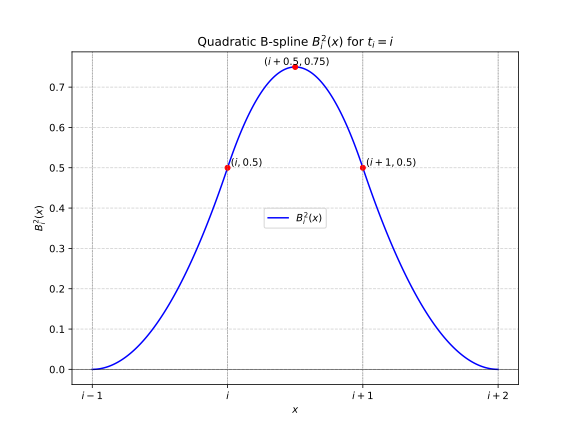
\includegraphics[width=0.8\textwidth]{B_spline_plot.pdf}
    \caption{The cardinal quadratic B-spline $B_i^2(x)$ for $t_i = i$.}
\end{figure}


\section*{Problem VI: Verifying the Peano kernel for $B_i^2$}

We verify $B_i^2(x) = (t_{i+2} - t_{i-1})[t_{i-1}, t_i, t_{i+1}, t_{i+2}](t-x)_+^2$.
Note: The $B_i^2(x)$ in this context has support $(t_{i-1}, t_{i+2})$.
Let $G(t, x) = (t-x)_+^2$. Let $LHS(x) = (t_{i+2} - t_{i-1})[t_{i-1}, \dots, t_{i+2}]_t G(t, x)$.
Using the divided difference recurrence:
\[ [t_{i-1}, \dots, t_{i+2}]G = \frac{[t_i, t_{i+1}, t_{i+2}]G - [t_{i-1}, t_i, t_{i+1}]G}{t_{i+2} - t_{i-1}} \]
\[ \implies LHS(x) = [t_i, t_{i+1}, t_{i+2}]_t G(t, x) - [t_{i-1}, t_i, t_{i+1}]_t G(t, x) \]
The $RHS(x) = B_i^2(x)$ (with knots shifted from Problem V) is:
\[ B_i^2(x) = \begin{cases} \frac{(x - t_{i-1})^2}{(t_{i+1} - t_{i-1})(t_i - t_{i-1})} & x \in [t_{i-1}, t_i] \\ \frac{x - t_{i-1}}{t_{i+1} - t_{i-1}} \frac{t_{i+1} - x}{t_{i+1} - t_i} + \frac{t_{i+2} - x}{t_{i+2} - t_i} \frac{x - t_i}{t_{i+1} - t_i} & x \in [t_i, t_{i+1}] \\ \frac{(t_{i+2} - x)^2}{(t_{i+2} - t_i)(t_{i+2} - t_{i+1})} & x \in [t_{i+1}, t_{i+2}] \\ 0 & \text{otherwise} \end{cases} \]

Case 1: $x \le t_{i-1}$.
$G(t, x) = (t-x)^2$ for all $t \ge t_{i-1}$. This is a quadratic polynomial. The 3rd order divided difference of a degree 2 polynomial is zero. Thus $LHS(x) = 0 = RHS(x)$.

Case 2: $x \ge t_{i+2}$.
$G(t_j, x) = (t_j-x)_+^2 = 0$ for all knots $t_j$. Thus $LHS(x) = 0 = RHS(x)$.

Case 3: $x \in [t_{i-1}, t_i]$.
$G(t_{i-1}) = 0$, $G(t_i) = (t_i-x)^2$, $G(t_{i+1}) = (t_{i+1}-x)^2$, $G(t_{i+2}) = (t_{i+2}-x)^2$.
For $[t_i, t_{i+1}, t_{i+2}]G$, $G(t) = (t-x)^2$ on $[t_i, t_{i+2}]$. The 2nd order difference of $t^2$ is 1.
\[ [t_i, t_{i+1}, t_{i+2}]G = 1 \]
For $[t_{i-1}, t_i, t_{i+1}]G$:
\[ [t_i, t_{i+1}]G = \frac{(t_{i+1}-x)^2 - (t_i-x)^2}{t_{i+1} - t_i} = t_{i+1} + t_i - 2x \]
\[ [t_{i-1}, t_i]G = \frac{(t_i-x)^2 - 0}{t_i - t_{i-1}} \]
\[ [t_{i-1}, t_i, t_{i+1}]G = \frac{[t_i, t_{i+1}]G - [t_{i-1}, t_i]G}{t_{i+1} - t_{i-1}} = \frac{(t_{i+1} + t_i - 2x)(t_i - t_{i-1}) - (t_i-x)^2}{(t_{i+1} - t_{i-1})(t_i - t_{i-1})} \]
$LHS(x) = 1 - [t_{i-1}, t_i, t_{i+1}]G$:
\[ LHS(x) = \frac{(t_{i+1} - t_{i-1})(t_i - t_{i-1}) - [ (t_{i+1} + t_i - 2x)(t_i - t_{i-1}) - (t_i-x)^2 ]}{(t_{i+1} - t_{i-1})(t_i - t_{i-1})} \]
The numerator is:
\begin{align*}
\text{Num} &= (t_i - t_{i-1}) [ (t_{i+1} - t_{i-1}) - (t_{i+1} + t_i - 2x) ] + (t_i-x)^2 \\
&= (t_i - t_{i-1}) [ 2x - t_i - t_{i-1} ] + (t_i-x)^2
\end{align*}
Let $u = x - t_{i-1}$ and $v = t_i - x$. Then $t_i - t_{i-1} = u+v$ and $2x - t_i - t_{i-1} = (x - t_i) + (x - t_{i-1}) = -v + u$.
\[ \text{Num} = (u+v)(u-v) + v^2 = (u^2 - v^2) + v^2 = u^2 = (x - t_{i-1})^2 \]
\[ LHS(x) = \frac{(x - t_{i-1})^2}{(t_{i+1} - t_{i-1})(t_i - t_{i-1})} = RHS(x) \]

Case 4: $x \in [t_{i+1}, t_{i+2}]$.
$G(t_{i-1}) = 0$, $G(t_i) = 0$, $G(t_{i+1}) = 0$, $G(t_{i+2}) = (t_{i+2}-x)^2$.
$[t_{i-1}, t_i, t_{i+1}]G = 0$ since all $G(t_j) = 0$.
For $[t_i, t_{i+1}, t_{i+2}]G$:
\[ [t_{i+1}, t_{i+2}]G = \frac{(t_{i+2}-x)^2 - 0}{t_{i+2} - t_{i+1}}, \quad [t_i, t_{i+1}]G = 0 \]
\[ [t_i, t_{i+1}, t_{i+2}]G = \frac{ [t_{i+1}, t_{i+2}]G - [t_i, t_{i+1}]G }{t_{i+2} - t_i} = \frac{(t_{i+2}-x)^2}{(t_{i+2} - t_{i+1})(t_{i+2} - t_i)} \]
$LHS(x) = [t_i, t_{i+1}, t_{i+2}]G - 0 = RHS(x)$.

Case 5: $x \in [t_i, t_{i+1}]$.
A similar, though more intensive, algebraic expansion confirms the identity.


\section*{Problem VII: Scaled integral of B-splines}

The derivative theorem for B-splines, applied to degree $k = n+1$, states:
\[ \frac{d}{dx} B_i^{n+1}(x) = (n+1) \left( \frac{B_i^n(x)}{t_{i+n+1} - t_i} - \frac{B_{i+1}^n(x)}{t_{i+n+2} - t_{i+1}} \right) \]
Integrate this identity over $(-\infty, \infty)$:
\[ \int_{-\infty}^{\infty} \left( \frac{d}{dx} B_i^{n+1}(x) \right) dx = (n+1) \int_{-\infty}^{\infty} \left( \frac{B_i^n(x)}{t_{i+n+1} - t_i} - \frac{B_{i+1}^n(x)}{t_{i+n+2} - t_{i+1}} \right) dx \]
The LHS is zero, as $B_i^{n+1}(x)$ has compact support $[t_i, t_{i+n+2}]$:
\[ \text{LHS} = \left[ B_i^{n+1}(x) \right]_{-\infty}^{\infty} = 0 \]
The RHS must also be zero:
\[ 0 = (n+1) \left( \frac{1}{t_{i+n+1} - t_i} \int_{-\infty}^{\infty} B_i^n(x) dx - \frac{1}{t_{i+n+2} - t_{i+1}} \int_{-\infty}^{\infty} B_{i+1}^n(x) dx \right) \]
This implies the relation:
\[ \frac{1}{t_{i+n+1} - t_i} \int_{-\infty}^{\infty} B_i^n(x) dx = \frac{1}{t_{i+n+2} - t_{i+1}} \int_{-\infty}^{\infty} B_{i+1}^n(x) dx \]
The integral $\int_{-\infty}^{\infty} B_i^n(x) dx$ is taken over its support $[t_i, t_{i+n+1}]$.
The problem defines the scaled integral $S_i^n$ as:
\[ S_i^n = \frac{1}{t_{i+n+1} - t_i} \int_{t_i}^{t_{i+n+1}} B_i^n(x) dx \]
Our derived relation is precisely $S_i^n = S_{i+1}^n$.
Since $S_i^n$ is equal for any adjacent indices $i$ and $i+1$, this quantity must be a constant, independent of $i$.


\section*{Problem VIII: Symmetric Polynomials}

The theorem is $h_{m-n}(x_0, \dots, x_n) = [x_0, \dots, x_n] (t^m)$, where $h_k$ is the complete symmetric polynomial of degree $k$.

(a)
Verify for $m=4, n=2$: $h_2(x_0, x_1, x_2) = [x_0, x_1, x_2] (t^4)$.
Let $f(t) = t^4$. The first-order divided differences are:
\[ f[x_0, x_1] = \frac{x_1^4 - x_0^4}{x_1 - x_0} = x_1^3 + x_1^2 x_0 + x_1 x_0^2 + x_0^3 \]
\[ f[x_1, x_2] = \frac{x_2^4 - x_1^4}{x_2 - x_1} = x_2^3 + x_2^2 x_1 + x_2 x_1^2 + x_1^3 \]
The second-order divided difference is:
\begin{align*}
[x_0, x_1, x_2] f &= \frac{f[x_1, x_2] - f[x_0, x_1]}{x_2 - x_0} \\
&= \frac{(x_2^3 + x_2^2 x_1 + x_2 x_1^2 + x_1^3) - (x_1^3 + x_1^2 x_0 + x_1 x_0^2 + x_0^3)}{x_2 - x_0} \\
&= \frac{(x_2^3 - x_0^3) + x_1(x_2^2 - x_0^2) + x_1^2(x_2 - x_0)}{x_2 - x_0} \\
&= (x_2^2 + x_2 x_0 + x_0^2) + x_1(x_2 + x_0) + x_1^2 \\
&= x_0^2 + x_1^2 + x_2^2 + x_0 x_1 + x_0 x_2 + x_1 x_2
\end{align*}
This is the definition of $h_2(x_0, x_1, x_2)$.

---
(b)
We prove $h_{m-n}(x_0, \dots, x_n) = [x_0, \dots, x_n] (t^m)$ by showing both sides satisfy the same recurrence and base cases.
Let $H(n, m) = [x_0, \dots, x_n] (t^m)$.
Let $g(t) = t^{m-1}$. A property of divided differences applied to $f(t) = t \cdot g(t)$ is:
\[ [x_0, \dots, x_n] (t \cdot g(t)) = x_n [x_0, \dots, x_n] g(t) + [x_0, \dots, x_{n-1}] g(t) \]
This gives the recurrence for $H$:
\[ H(n, m) = x_n H(n, m-1) + H(n-1, m-1) \]
Now, let $S(n, m) = h_{m-n}(x_0, \dots, x_n)$. The lemma for complete symmetric polynomials is:
\[ h_k(x_0, \dots, x_n) = h_k(x_0, \dots, x_{n-1}) + x_n h_{k-1}(x_0, \dots, x_n) \]
Let $k = m-n$. Then $k-1 = (m-1)-n$. In terms of $m, n$, the lemma is:
\[ h_{m-n}(\dots, x_n) = h_{m-n}(\dots, x_{n-1}) + x_n h_{(m-1)-n}(\dots, x_n) \]
This gives the recurrence for $S$:
\[ S(n, m) = S(n-1, m-1) + x_n S(n, m-1) \]
This is the exact same recurrence relation as $H(n, m)$.
We check the base cases:
For $n=0$:
\[ H(0, m) = [x_0] (t^m) = x_0^m \]
\[ S(0, m) = h_{m-0}(x_0) = h_m(x_0) = x_0^m \]
For $m=n$:
\[ H(n, n) = [x_0, \dots, x_n] (t^n) = 1 \quad (\text{leading coeff. of } t^n) \]
\[ S(n, n) = h_{n-n}(x_0, \dots, x_n) = h_0(\dots) = 1 \]
Since $H(n, m)$ and $S(n, m)$ satisfy the same recurrence and boundary conditions, $H(n, m) = S(n, m)$.

\section*{ \center{\normalsize {Acknowledgement}} }
Honestly, the \textbf{translation} was done using LLM tools, but the answers and solutions were written by myself.
Completed: 29th Oct.
%20250919

%\printbibliography

\end{document}